\appendix

\section{Equations and parameters of the benchmark systems}\label{app:systems}

\textbf{Chua circuit:}\cite{Leonov2011PLA,GuanXie2025}
\begin{equation*}
\begin{split}
&\dot x=\alpha\bigl(y-x-f(x)\bigr),\quad \dot y=x-y+z,\\
&\dot z=-(\beta y+\gamma z),\\
&f(x)=m_1x+\tfrac12(m_0-m_1)\bigl(|x+1|-|x-1|\bigr).
\end{split}
\end{equation*}
The parameters $(\alpha,\beta,\gamma,m_0,m_1)$ are
\begin{equation*}
\begin{split}
&\text{set I: } (8.4562,\ 12.0732,\ 0.0052,\ -0.1768,\ -1.1468),\\
&\text{set II: } (8.4,\ 12,\ -0.005,\ -1.2,\ -0.05).
\end{split}
\end{equation*}
For set II, the known regimes are the cycle LC passing through $(-7.287,-2.773,36.02)$ and the chaotic attractors passing through $(1.528,0.283,-1.819)$ and $(-1.304,0.029,2.387)$. Two coupled circuits (Sec.~\ref{sec:coupled}): $\dot x_u=\alpha(y_u-x_u-f(x_u))+\epsilon(\bar x-x_u)$, $\bar x=(x_1+x_2)/2$, with the other equations unchanged, in the region $B^2$.

\textbf{Systems without equilibria.} NE4: $\dot x=-0.1y+a$, $\dot y=x+z$, $\dot z=xz-3y$, $a=1$. Wang--Chen \#1:\cite{WangChen2012} $\dot x=y$, $\dot y=z$, $\dot z=-y+3y^2-x^2-xz+a$, $a=-0.05$. Wei:\cite{Wei2011} $\dot x=-y$, $\dot y=cx+z$, $\dot z=ay^2+xz-d$, $(a,c,d)=(2,1,0.35)$. Jafari \textit{et al.} 2026:\cite{Jafari2026NoPP} $\dot x=y$, $\dot y=z$, $\dot z=a_1z+a_2xy+a_3yz+a_4zx+a_5$, $(a_1,a_2,a_4,a_5)=(6,-1,-1,-1)$; a cycle at $a_3=-1$ and chaos at $a_3=-3.548$, with the state $(6.7445,0.4214,-1.7846)$ on the attractor.

\textbf{A single stable equilibrium.} Wang--Chen \#2:\cite{WangChen2012} $\dot x=yz+a$, $\dot y=x^2-y$, $\dot z=1-4x$, $a=0.006$. SE3:\cite{Molaie2013} $\dot x=y$, $\dot y=z$, $\dot z=-3.4x-y-4z+y^2+xy$. SE11:\cite{Molaie2013} $\dot x=y$, $\dot y=-x+yz$, $\dot z=-y-12z+x^2+9xz-1$.

\textbf{A line of equilibria.} LE1:\cite{JafariSprott2013} $\dot x=y$, $\dot y=-x+yz$, $\dot z=-x-axy-bxz$, $(a,b)=(15,1)$; the equilibria $(0,0,z)$ are stable for $z<0$.

\textbf{Rabinovich system:}\cite{Kuznetsov2018Rabinovich} $\dot x=-\sigma(x-y)-ayz$, $\dot y=rx-y-xz$, $\dot z=-bz+xy$, $\sigma=-ar$; $(r,a,b)=(100,-0.009965,0.077454)$ (hidden attractor) and $(6.8,-0.5,0.99)$ (transient set\cite{SprottMunmuangsaen2018Comment}).

\textbf{Negative control.} The Lorenz system $\dot x=a(y-x)$, $\dot y=rx-y-xz$, $\dot z=xy-bz$ at $(a,r,b)=(4,29,2)$.

\textbf{Maps.} Huynh \textit{et al.}:\cite{Huynh2019} $x'=x+y$, $y'=y-a|y|-xy+bx^2-cy^2+d$, $(a,b,c,d)=(0.01,0.1,2,0.1)$. General family of Jiang \textit{et al.}:\cite{Jiang2016Maps} $x'=y$, $y'=a_1x+a_2y+a_3x^2+a_4y^2+a_5xy+a_6$; the cases used and their coefficients $(a_1,\dots,a_6)$ are listed below.
\begin{itemize}
\item NF I e: $(1,0,0,-0.3,0.3,2.98)$, box $[-8,8]^2$.
\item NF I f: $(1,0,0,0.38,-0.38,-1.6)$, box $[-5,5]^2$.
\item NF I g: $(1,0,0,0.12,-0.12,-3.62)$, box $[-8,8]^2$.
\item NF I i: $(1,0,0,-0.3,0.3,1.09)$, box $[-5,5]^2$.
\item SF I a: $(-0.33,0.17,-0.48,0.47,0.01,-0.9)$, box $[-5,5]^2$.
\item SF I b: $(-0.84,0,0,0.15,-0.15,-5.85)$, box $[-12,12]^2$.
\item SF I c: $(-0.99,0,0,0.23,-0.23,-4.24)$, box $[-10,10]^2$.
\item SF I d: $(-1.29,2,-0.35,-0.85,1.2,0.17)$, box $[-5,5]^2$.
\end{itemize}
The same family in the form of Ref.~\onlinecite{Ouannas2018}: $x'=y$, $y'=x+a_1x^2+a_2y^2-a_3xy-a_4$, with the parameter sets $(0.2,0.71,0.91,1.14)$, $(0.51,1,1.51,0.74)$, and $(0.6,1,1.6,0.72)$ (``Jiang--Ouannas 1--3'' in Table~\ref{tab:integration}).

\textbf{Four-dimensional systems.} Li and Sprott:\cite{LiSprott2014} $\dot x=y-x$, $\dot y=-xz+u$, $\dot z=xy-a$, $\dot u=-by$ at $(a,b)=(6,0.1)$, $(7,0.1)$, and $(2.6,0.44)$. Jahanshahi \textit{et al.}:\cite{Jahanshahi2019} $\dot x=y$, $\dot y=z$, $\dot z=w$, $\dot w=-aw+bx^2-cy^2+exy+fxz+g$, $(a,b,c,e,f,g)=(1.05,0.7,0.19,1.37,1.79,1.15)$.

\textbf{Synthetic families} D1 and D2: Eqs.~\eqref{eq:d1} and \eqref{eq:d2} with the base SE3, $B=[-10,10]^3\times[-1,1]^m$, $m=1$--11, integrated with the settings of SE3; in D2, the transient segment is extended by $\ln(\sqrt m/\rho)/\kappa+5$ time units so that every escaping trajectory leaves before the observation window.

The integration parameters and the regions of initial conditions are listed in Table~\ref{tab:integration}; the control systems are included. Figure~\ref{fig:chuaI} shows the Chua circuit with parameter set I, Fig.~\ref{fig:jafari} the chaos window of the Jafari 2026 system, Fig.~\ref{fig:maps} the level-B maps, and Fig.~\ref{fig:levelA} the level-C system of Li and Sprott.

\begin{table*}
\caption{Integration parameters and regions of initial conditions $B$. For flows, the lengths of the transient segment and of the observation window are given in time units, and for maps in iterations; $R_{\rm esc}$ is the escape threshold.}
\label{tab:integration}
\begin{ruledtabular}
\begin{tabular}{lrlrlr}
System & $n$ & Integration & $T_{\rm tr}/T_{\rm obs}$ & Region $B$ & $R_{\rm esc}$ \\
\hline
Chua I & 3 & RK4, $\Delta t=0.0025$ & 1000 / 100 & $[-10,10]^2\times[-15,15]$ & 100 \\
Chua II & 3 & RK4, $\Delta t=0.0025$ & 1000 / 100 & $[-10,10]^2\times[-15,15]$ & 100 \\
NE4 & 3 & RK4, $\Delta t=0.001$ & 500 / 500 & $[-40,20]\times[-30,50]\times[-80,220]$ & 2000 \\
Wang--Chen \#1 & 3 & RK4, $\Delta t=0.01$ & 300 / 100 & $[-10,10]^3$ & 100 \\
Wei (NE2) & 3 & RK4, $\Delta t=0.01$ & 300 / 100 & $[-10,10]^3$ & 100 \\
Jafari 2026, $a_3=-1$ & 3 & RK4, $\Delta t=0.01$ & 3000 / 200 & $[-10,10]^3$ & 60 \\
Jafari 2026, $a_3=-3.548$ & 3 & RK4, $\Delta t=0.005$ & 1000 / 200 & $[-10,10]^3$ & 60 \\
Wang--Chen \#2 & 3 & RK4, $\Delta t=0.01$ & 300 / 100 & $[-10,10]^3$ & 100 \\
SE3 & 3 & RK4, $\Delta t=0.01$ & 300 / 100 & $[-10,10]^3$ & 100 \\
SE11 & 3 & RK4, $\Delta t=0.01$ & 300 / 100 & $[-10,10]^3$ & 100 \\
LE1 & 3 & RK4, $\Delta t=0.01$ & 300 / 100 & $[-10,10]^3$ & 100 \\
Rabinovich, $r=100$ & 3 & RK4, $\Delta t=0.002$ & 200 / 100 & $[-60,60]^2\times[-150,150]$ & 1000 \\
Rabinovich, $r=6.8$ & 3 & RK4, $\Delta t=0.005$ & 300 / 100 & $[-10,10]^2\times[-10,15]$ & 200 \\
Lorenz $(4,29,2)$ & 3 & RK4, $\Delta t=0.005$ & 300 / 100 & $[-20,20]^2\times[0,50]$ & 500 \\
D1, D2 (base SE3) & $3+m$ & RK4, $\Delta t=0.01$ & $\ge300$ / 100 & $[-10,10]^3\times[-1,1]^m$ & 100 \\
Huynh 2019 & 2 & iterations & 20\,000 / 5000 & $[-3,3]^2$ & 100 \\
Jiang NF I e & 2 & iterations & 20\,000 / 5000 & $[-8,8]^2$ & 1000 \\
Jiang NF I f & 2 & iterations & 20\,000 / 5000 & $[-5,5]^2$ & 1000 \\
Jiang NF I g & 2 & iterations & 20\,000 / 5000 & $[-8,8]^2$ & 1000 \\
Jiang NF I i & 2 & iterations & 20\,000 / 5000 & $[-5,5]^2$ & 1000 \\
Jiang SF I a & 2 & iterations & 20\,000 / 5000 & $[-5,5]^2$ & 1000 \\
Jiang SF I b & 2 & iterations & 20\,000 / 5000 & $[-12,12]^2$ & 1000 \\
Jiang SF I c & 2 & iterations & 20\,000 / 5000 & $[-10,10]^2$ & 1000 \\
Jiang SF I d & 2 & iterations & 20\,000 / 5000 & $[-5,5]^2$ & 1000 \\
Jiang--Ouannas 1--3 & 2 & iterations & 20\,000 / 5000 & $[-2,2]^2$ & 100 \\
H\'enon (control) & 2 & iterations & 5000 / 2000 & $[-2,2]^2$ & 50 \\
Li--Sprott 4D, $a=6$ & 4 & RK4, $\Delta t=0.005$ & 500 / 200 & $[-15,15]^4$ & 500 \\
Li--Sprott 4D, $a=7$ & 4 & RK4, $\Delta t=0.005$ & 500 / 200 & $[-15,15]^4$ & 500 \\
Li--Sprott 4D, hyperchaos & 4 & RK4, $\Delta t=0.005$ & 500 / 200 & $[-15,15]^4$ & 500 \\
Jahanshahi 4D & 4 & RK4, $\Delta t=0.005$ & 500 / 200 & $[-10,10]^4$ & 500 \\
Coupled Chua II, $\epsilon=0.1$ & 6 & RK4, $\Delta t=0.0025$ & 1000 / 100 & $\bigl([-10,10]^2\times[-15,15]\bigr)^2$ & 141 \\
\end{tabular}
\end{ruledtabular}
\end{table*}

\begin{figure*}
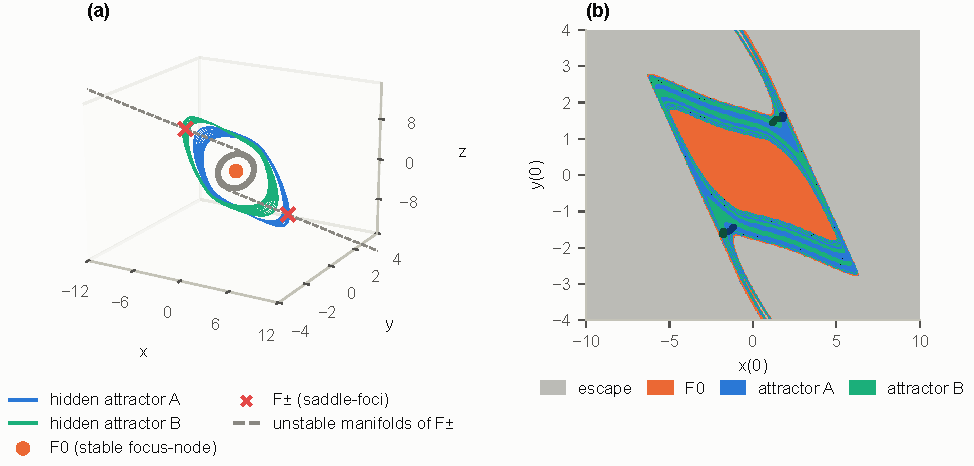
\includegraphics[width=\textwidth]{figures/fig30_chua_I_hidden.pdf}
\caption{Chua circuit, parameter set I. (a) Two symmetric hidden chaotic attractors A and B, the stable focus-node F$_0$ (dot), the saddle-foci F$_\pm$ (crosses), and their unstable manifolds. One branch of each manifold escapes to infinity and the other winds onto F$_0$, so the standard procedure does not find attractors A and B. (b) Basins in the plane $z(0)=0$ (window $|y|\le4$). Gray: escape to infinity; orange: F$_0$; blue and green: attractors A and B.}
\label{fig:chuaI}
\end{figure*}

\begin{figure}
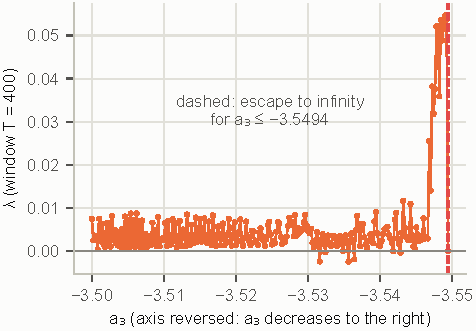
\includegraphics[width=\columnwidth]{figures/fig35_jafari2026.pdf}
\caption{System of Jafari \textit{et al.}\cite{Jafari2026NoPP} without fixed and perpetual points: the Lyapunov exponent over windows $T=400$ in the narrow chaos window near the boundedness limit ($a_3$ decreases to the right); for $a_3\le-3.5494$, trajectories escape to infinity. The cycle at $a_3=-1$ and the chaotic attractor at $a_3=-3.548$ are shown in Fig.~\ref{fig:gallery3d}.}
\label{fig:jafari}
\end{figure}

\begin{figure*}
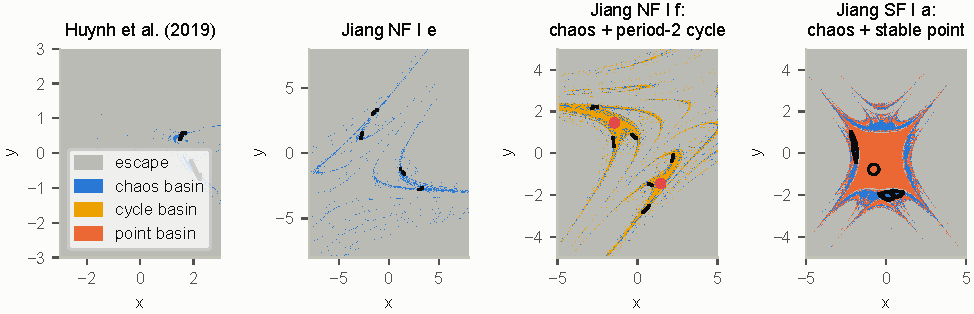
\includegraphics[width=\textwidth]{figures/fig34_maps_phase_basin.pdf}
\caption{Two-dimensional maps of level B: phase--basin portraits. (a) The map of Huynh \textit{et al.}\cite{Huynh2019} without fixed points ($p=0.0091$ in $[-3,3]^2$). (b), (c) Cases NF~I~e and NF~I~f of the family of Jiang \textit{et al.}\cite{Jiang2016Maps} without fixed points; in NF~I~f, a chaotic attractor coexists with a period-2 cycle (markers). (d) Case SF~I~a with a single stable fixed point (circle). Light gray: escape; dark blue: basin of the chaotic attractor; white: basin of the cycle; orange: basin of the fixed point; black: the attractor.}
\label{fig:maps}
\end{figure*}

\begin{figure*}
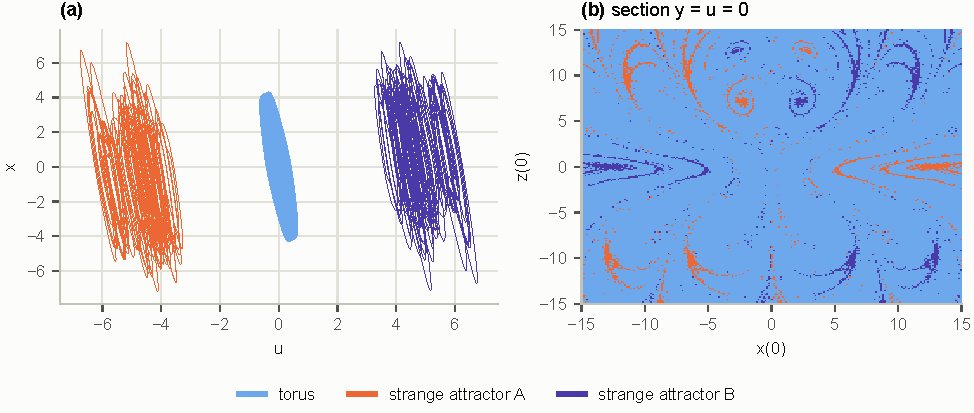
\includegraphics[width=\textwidth]{figures/fig33_li_sprott_4d.pdf}
\caption{Four-dimensional simplified Lorenz system\cite{LiSprott2014} at $a=6$, $b=0.1$; there are no equilibria. (a) The torus (basin fraction 0.090) and a pair of symmetric strange attractors ($\lambda\approx0.25$; 0.446 and 0.464) in the projection $(u,x)$. (b) Basins in the section $y=u=0$ of the box $[-15,15]^4$; the torus occupies the ``background,'' and the strange attractors form spiral tongues. Here the rare target is the torus, not the chaos.}
\label{fig:levelA}
\end{figure*}

\section{Verification episodes}\label{app:verification}

This appendix documents the three cases mentioned in Sec.~\ref{sec:protocol} and the measured hiddenness.

\textbf{Numerical ``transient chaos'' in the Chua circuit.} With RK4 at $\Delta t=0.01$, all 256 copies of a state on the hidden chaotic set of Chua~I converge within $t\le2\times10^4$ to a spurious periodic orbit of the same size (median time about 1500; Fig.~\ref{fig:chuatrans}a). At $\Delta t=0.0025$, none of 96 copies leaves before $t=10^4$, and DOP853 preserves the chaos up to $t=4000$. At $\Delta t=0.01$, the fractions of the hidden attractors are underestimated almost twofold (Fig.~\ref{fig:chuatrans}b). For a piecewise-linear system, this is an integrator artifact and the mirror image of the spurious ``hidden Lorenz attractor'':\cite{Munmuangsaen2018,SprottMunmuangsaen2018Comment} there, transient chaos was mistaken for an attractor; here, an attractor is mistaken for transient chaos. The step-convergence check is therefore mandatory.

\textbf{Basin fractions of the Chua circuit.} Two independent implementations, Python (RK4, $\Delta t=0.0025$) and Attractors.jl (Vern9), give identical fractions in the balls $r=3$ and $r=5$ and in Zelinka's box. Neither of them reproduces Table~1 of the review in Ref.~\onlinecite{GuanXie2025} (Table~\ref{tab:chuafrac}). In the ball $r=3$, the escape fraction is 0.19 in our computations versus 0.06 in the review, the fraction of F$_0$ is 0.44 versus 0.75, and that of each hidden attractor is 0.18 versus 0.095. The last pair is suggestive: our fractions of the hidden attractors at the coarse step $\Delta t=0.01$ are also about 0.09 (Fig.~\ref{fig:chuatrans}b), so the review's values are consistent with the artifact above, whereas its escape and F$_0$ fractions remain unexplained. The basin structure in the plane $z=0$ coincides with the review and with the catalog of Ref.~\onlinecite{Wagemakers2025Zoo} (Fig.~\ref{fig:chuaI}).

\textbf{Intermittency and transient sets.} In NE4, the ``second attractor'' of a preliminary version of the protocol turned out to be intermittency of the single chaotic attractor; this was fixed by the window $T_{\rm obs}=500\gg1/\lambda$. The transient chaos of the Lorenz system $(4,29,2)$ lives about $10^4$ time units: all eight copies decay by $t\le7\times10^4$. A protocol with an observation window shorter than the lifetime would accept this set as an attractor (Fig.~\ref{fig:verif}). The Rabinovich set at $r=6.8$ lives longer than $10^5$ for six of eight copies, consistent with the estimate $\tau\sim5\times10^7$ of Ref.~\onlinecite{SprottMunmuangsaen2018Comment}; in the benchmark, it is used only as a control.

\textbf{Hiddenness measure.} Table~\ref{tab:hidden} lists $h_\varepsilon$ for the systems with equilibria. For SE3 and SE11, $h_\varepsilon=0$ at all three scales. For Chua~I, $h_\varepsilon$ grows from 0 at $\varepsilon=10^{-3}L$ through 0.003 ($10^{-2}L$) to 0.19 ($10^{-1}L$). For the Rabinovich system at $r=100$, the values are 0, 0.03, and 0.65: the attractor is hidden only in the strict limit $\varepsilon\to0$, and already at $\varepsilon=10^{-2}L$, trajectories from the neighborhood of an equilibrium enter its basin. The binary definition thus does not distinguish ``deeply'' and ``shallowly'' hidden attractors, whereas $h_\varepsilon$ does. For the Jafari chaos, whose copies with a perturbation of $10^{-3}$ escape (Fig.~\ref{fig:verif}), all 32 copies with a perturbation of $10^{-6}$ stay on the attractor for $10^4$ time units with RK4, and so do eight copies with DOP853, with finite-time exponents of $0.056\pm0.011$ and none below 0.01: it is an attractor with a basin thinner than a relative distance of $10^{-3}$ near the attractor, not a long transient.

A measured zero of $h_\varepsilon$ is informative only relative to the number of starts $n$: with no hits, $h_\varepsilon<3/n$ at the 95\% level, so the zeros of Table~\ref{tab:hidden} bound $h_\varepsilon$ by the values given there, and for the rare targets with $p$ comparable to $3/n$ the zero does not by itself separate ``hidden'' from ``rare.'' For SE11, Chua~II, and the rare family of the coupled Chua circuits, the measure was therefore remeasured with $2\times10^5$ starts per radius: no start reaches a hidden target at $10^{-3}L$ or $10^{-2}L$, so $h_\varepsilon<1.5\times10^{-5}$ at the 95\% level, below the basin measures of all three targets (Sec.~\ref{sec:coupled}).

% Proposed caption (replaces the bar chart fig04_table1_comparison / \ref{fig:table1}):
% Basin fractions of Chua~I under uniform sampling in balls of radius $r=3$ and $r=5$ about the origin: escape to infinity ($\infty$), the stable equilibrium F$_0$, and the two symmetric hidden attractors A and B. Sources: Table~1 of the review in Ref.~\onlinecite{GuanXie2025} and two independent implementations, Python (RK4, $dt=0.0025$, $10^5$ points per ball) and Attractors.jl (Vern9, $10^4$ points per ball). The two implementations agree with each other but not with the review. In the implementations, A and B are matched by the sign of the mean of $x$ on the attractor; for the review, they are listed in the order of its Table~1. The fraction of unmatched trajectories in the Python run (0.06\%) is omitted.

\begin{table}
\caption{Basin fractions of Chua~I under uniform sampling in balls of radius $r=3$ and $r=5$ about the origin: escape to infinity ($\infty$), the stable equilibrium F$_0$, and the two symmetric hidden attractors A and B. Sources: Table~1 of the review in Ref.~\onlinecite{GuanXie2025} and two independent implementations, Python (RK4, $dt=0.0025$, $10^5$ points per ball) and Attractors.jl (Vern9, $10^4$ points per ball). The two implementations agree with each other but not with the review. In the implementations, A and B are matched by the sign of the mean of $x$ on the attractor; for the review, they are listed in the order of its Table~1. The fraction of unmatched trajectories in the Python run (0.06\%) is omitted.}
\label{tab:chuafrac}
\footnotesize
\setlength{\tabcolsep}{3pt}
\begin{ruledtabular}
\begin{tabular}{lrrrrrrrr}
 & \multicolumn{4}{c}{$r=3$} & \multicolumn{4}{c}{$r=5$} \\
Source & $\infty$ & F$_0$ & A & B & $\infty$ & F$_0$ & A & B \\
\hline
Ref.~\onlinecite{GuanXie2025}, Table~1 & 0.06 & 0.75 & 0.09 & 0.10 & 0.23 & 0.50 & 0.14 & 0.13 \\
Python, RK4 & 0.19 & 0.44 & 0.18 & 0.18 & 0.55 & 0.18 & 0.14 & 0.14 \\
Attractors.jl & 0.19 & 0.44 & 0.18 & 0.19 & 0.55 & 0.18 & 0.13 & 0.14 \\
\end{tabular}
\end{ruledtabular}
\end{table}


% Proposed caption (replaces the plot fig40_hiddenness / \ref{fig:hidden}):
% Hiddenness measure $h_\varepsilon$: the fraction of trajectories started in the $\varepsilon$-neighborhoods of the equilibria (uniformly in the ball of radius $\varepsilon$ about each equilibrium, plus the two points $e\pm\varepsilon u$ along every unstable eigendirection $u$) that enter the basin of the attractor, for $\varepsilon=10^{-3}L$, $10^{-2}L$, and $10^{-1}L$, where $L$ is the half-width of the region $B$; $n$ is the number of starts per radius. An entry 0 means no hit among the $n$ starts (95\% upper bound $3/n$). For Chua~I and Chua~II, the two hidden attractors are listed separately; the values quoted in the text for Chua~I are the sums over A and B. The Lorenz transient set is shown for comparison.
% Data caveat (results/e11_hiddenness.json): the reference set of this experiment contains one chaotic attractor of Chua II
% (new1) and the cycle LC (new0); at eps = 1e-1 L, 103 of 1202 starts (8.6%) reach an unmatched regime, presumably the
% symmetric second chaotic attractor, so h for "chaos, both" would be about 0.18. Wang--Chen #2 at 1e-1 L: 2 unmatched, 1% escape.
% Hits behind the nonzero entries: Chua I A 3/101, B 1/122 (1e-2 L / 1e-1 L); Chua II LC 484, chaos 115; Rabinovich 39/781;
% Lorenz 49.

\begin{table}
\caption{Hiddenness measure $h_\varepsilon$: the fraction of trajectories started in the $\varepsilon$-neighborhoods of the equilibria (uniformly in the ball of radius $\varepsilon$ about each equilibrium, plus the two points $e\pm\varepsilon u$ along every unstable eigendirection $u$) that enter the basin of the attractor, for $\varepsilon=10^{-3}L$, $10^{-2}L$, and $10^{-1}L$, where $L$ is the half-width of the region $B$; $n$ is the number of starts per radius. An entry 0 means no hit among the $n$ starts (95\% upper bound $3/n$). For Chua~I and Chua~II, the two hidden attractors are listed separately; the values quoted in the text for Chua~I are the sums over A and B. The Lorenz transient set is shown for comparison.}
\label{tab:hidden}
\footnotesize
\begin{ruledtabular}
\begin{tabular}{lrrrr}
System, attractor & $n$ & $\varepsilon=10^{-3}L$ & $10^{-2}L$ & $10^{-1}L$ \\
\hline
Chua I, A & 1204 & 0 & 0.00249 & 0.0839 \\
Chua I, B & 1204 & 0 & 0.000831 & 0.101 \\
Chua II, cycle LC & 1202 & 0 & 0 & 0.403 \\
Chua II, chaos & 1202 & 0 & 0 & 0.0957 \\
Wang--Chen \#2 & 400 & 0 & 0 & 0.838 \\
SE3 & 400 & 0 & 0 & 0 \\
SE11 & 400 & 0 & 0 & 0 \\
Rabinovich, $r=100$ & 1202 & 0 & 0.0324 & 0.650 \\
Lorenz $(4,29,2)$, transient set & 1202 & 0 & 0 & 0.0408 \\
\end{tabular}
\end{ruledtabular}
\end{table}


\begin{figure}
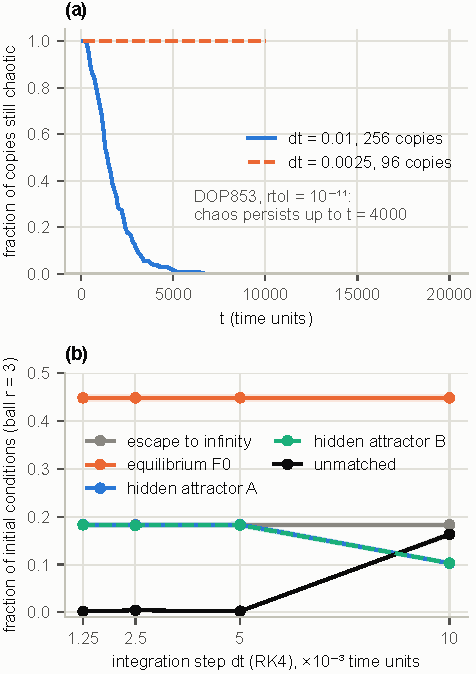
\includegraphics[width=\columnwidth]{figures/fig02_chua_transient.pdf}
\caption{Numerical ``transient chaos'' in Chua~I. (a) The fraction of copies (initial perturbation $10^{-3}$) remaining on the hidden chaotic set. With RK4 at $\Delta t=0.01$, the chaos decays onto a spurious periodic orbit; at $\Delta t=0.0025$, it persists to the end of the window. (b) Basin fractions versus the RK4 step (ball $r=3$, $2\times10^4$ points, $T_{\rm tr}=1000$). At $\Delta t=0.01$, about 16\% of trajectories land on the spurious orbit (``unmatched''), and the fractions of the hidden attractors are underestimated. For $\Delta t\le0.005$, the fractions stabilize.}
\label{fig:chuatrans}
\end{figure}

\begin{figure*}
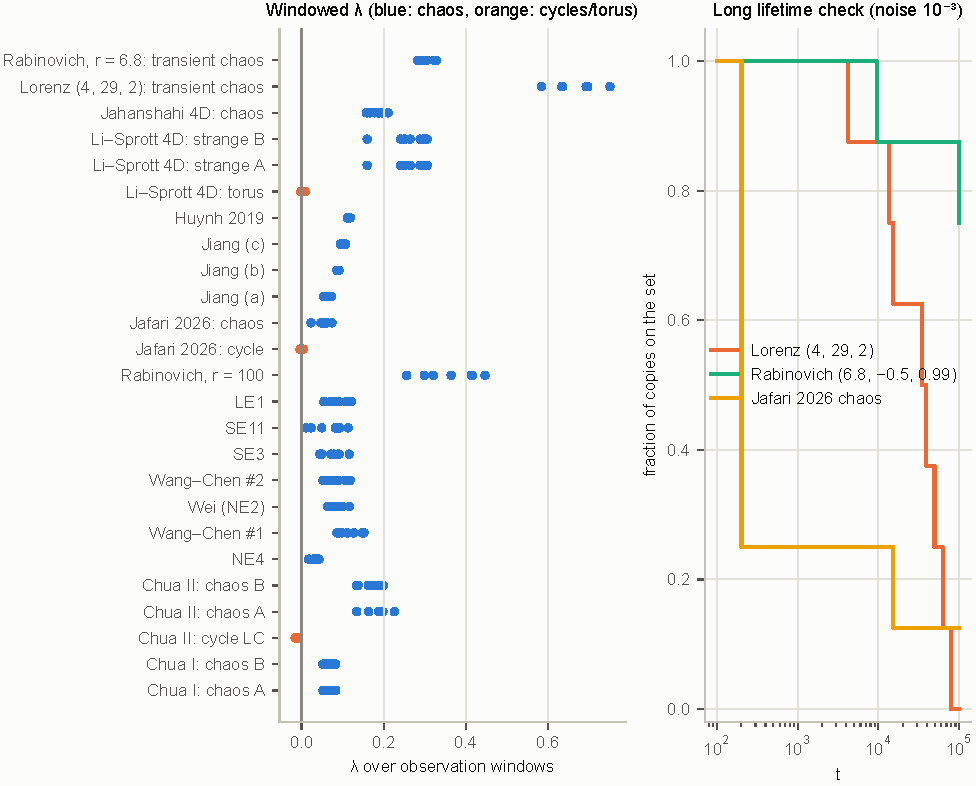
\includegraphics[width=\textwidth]{figures/fig41_verification.pdf}
\caption{Verification of the targets. (a) The largest Lyapunov exponent over consecutive observation windows for all targets of the benchmark; blue: chaotic regimes; orange: regular ones (cycle LC of Chua~II, the Jafari cycle, the Li--Sprott torus). (b) Long lifetime check (eight copies with initial perturbation $10^{-3}$). The Lorenz transient chaos decays completely. For the Rabinovich set at $r=6.8$, six of eight copies survive to $10^5$. For the fragile Jafari chaos, six of eight copies escape to infinity already by $t=200$: with a relative perturbation of $10^{-3}$, the copies leave its thin basin; with $10^{-6}$, all of them stay on the attractor (Appendix~\ref{app:verification}).}
\label{fig:verif}
\end{figure*}

\section{Classical heuristics}\label{app:classic}

The classical heuristics behave on the benchmark in agreement with the review in Ref.~\onlinecite{GuanXie2025} (Table~\ref{tab:classic}). Perpetual points lead to the target in Wang--Chen \#1, Wei, and Rabinovich. The Chua circuit has none: in the linear zones, the acceleration vanishes only at equilibria. They are also absent in SE3, SE11, and Wang--Chen \#2, while in NE4 and LE1 they exist but do not lead to the target. Sampling on nullclines (coordinate-wise zero-velocity sets\cite{Godara2018CVS}) gives gains in hit frequency from 1.1 (SE11) and 2.6 (LE1) to 4.5 (Chua~I). Connecting curves\cite{GuanXie2021CC} gain a factor of 2 in Wang--Chen \#1 and give no hits in SE3 and SE11. Continuation from the describing function finds the target in Chua~I within 10 integrations but applies only to Lur'e-type systems.

% Proposed caption (replaces the bar chart fig07_classic_vs_uniform / \ref{fig:classic}):
% Classical heuristics versus uniform sampling on the level-A targets: the number of integrations to detection with probability 0.9, $N_{0.9}=\lceil\ln0.1/\ln(1-p)\rceil$, where $p$ is the hit frequency of the sampling scheme. Uniform: sampling in $B$ ($p$ from $2\times10^4$ points; the geometric value, which differs slightly from the measured $N^0_{0.9}$ of Table~\ref{tab:gains}). CVS: sampling on the coordinate-wise zero-velocity sets (nullclines) $\dot x_i=0$, up to $10^3$ points on each, best coordinate. CC: sampling on connecting curves, 400 points. ``Not found'': no hit among the sampled points. PP: the number of perpetual points that lead to the target over the number of perpetual points found (``none'': the system has no perpetual points).

\begin{table}
\caption{Classical heuristics versus uniform sampling on the level-A targets: the number of integrations to detection with probability 0.9, $N_{0.9}=\lceil\ln0.1/\ln(1-p)\rceil$, where $p$ is the hit frequency of the sampling scheme. Uniform: sampling in $B$ ($p$ from $2\times10^4$ points; the geometric value, which differs slightly from the measured $N^0_{0.9}$ of Table~\ref{tab:gains}). CVS: sampling on the coordinate-wise zero-velocity sets (nullclines) $\dot x_i=0$, up to $10^3$ points on each, best coordinate. CC: sampling on connecting curves, 400 points. ``Not found'': no hit among the sampled points. PP: the number of perpetual points that lead to the target over the number of perpetual points found (``none'': the system has no perpetual points).}
\label{tab:classic}
\footnotesize
\setlength{\tabcolsep}{3pt}
\begin{ruledtabular}
\begin{tabular}{lrrrr}
Target & Uniform & CVS & CC & PP \\
 & $N^0_{0.9}$ & $N_{0.9}$ & $N_{0.9}$ & hits/total \\
\hline
Rabinovich, $r=100$ & 2 & 2 & 2 & 2/2 \\
Wang--Chen \#2 & 3 & 1 & 2 & none \\
NE4 & 6 & 7 & 29 & 0/1 \\
SE3 & 14 & 11 & not found & none \\
Wang--Chen \#1 & 22 & 19 & 11 & 1/2 \\
Wei (NE2) & 23 & 17 & 22 & 1/2 \\
Chua I, chaos A\footnotemark[1] & 136 & 14 & 172 & none \\
Chua I, chaos B\footnotemark[1] & 124 & 14 & 172 & none \\
SE11 & 291 & 255 & not found & none \\
LE1 & 1475 & 575 & 920 & 0/1 \\
\end{tabular}
\end{ruledtabular}
\footnotetext[1]{The heuristics count hits on either of the two hidden attractors; the uniform cost for either attractor is 65.}
\end{table}


\section{Ablation, baselines, and robustness}\label{app:ablation}

\textbf{Ablation.} The contributions of the components are shown in Fig.~\ref{fig:ablation}. On Chua~II, the arms add up: the portfolio gives 7.4 times, versus 5.1 for splitting and 3.2 for active learning. On LE1, the active-learning arm hurts, and the gain of the portfolio is provided by the splitting arm. Without the uniform share, the portfolio is not faster (Chua~II: 7.0; SE11: 3.1; LE1: 5.1) and loses where there is no signal (Jafari cycle: 0.27 against 0.43). On LE1, the lower interval bound for $G$ without the uniform share is 1.59, whereas for the portfolio with $\theta=0.2$, it is 3.76. Multidimensional ``rarity'' as a reaction coordinate produces heavy tails: the chains get stuck in atypical but nontarget regions, for example, in the basin of an equilibrium inside the D2 ball. The escape step as a coordinate is equivalent to $\xi$ everywhere except Chua~II, where all trajectories are bounded and it gives 1.04 against 5.05. Two earlier strategies were also tested ($R=20$): adaptive multilevel splitting driven by the novelty of the asymptotic fingerprint finds the target on Chua~II in only 55\% of runs, and MAP-Elites with the fingerprint as behavior descriptor has a median 5.6 times better than uniform sampling but a heavy tail, $G=0.36$. Such tails are what the uniform share of the portfolio removes.

\begin{figure*}
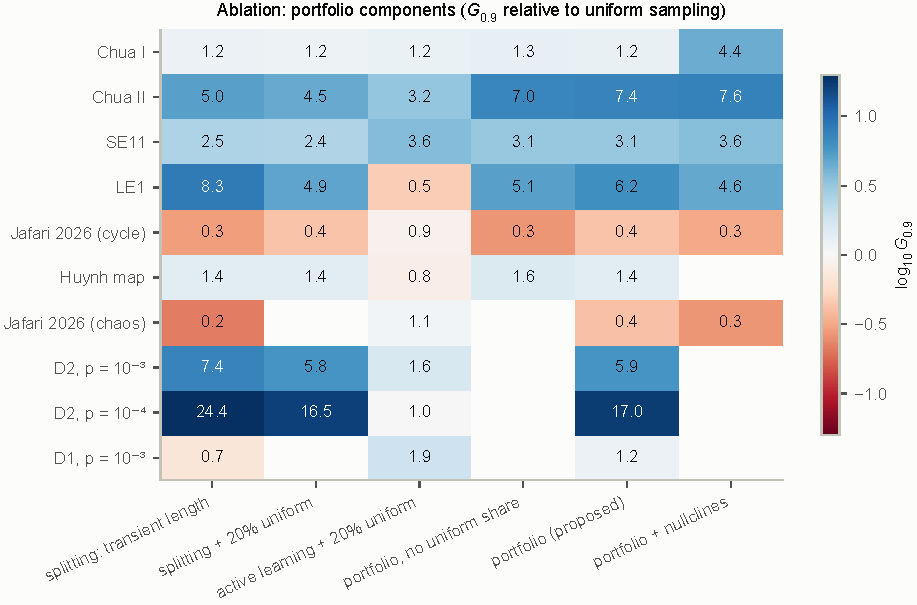
\includegraphics[width=\textwidth]{figures/fig25_ablation.pdf}
\caption{Ablation: $G_{0.9}$ of the variants of the method relative to uniform sampling ($R=100$; color: $\log_{10}G$; empty cells: the variant was not run). Rows: systems of levels A and B and synthetic families; columns: splitting alone and with a uniform share, active learning with a uniform share, the portfolio without a uniform share, the portfolio, and the portfolio with nullclines. Columns 1, 3, 5, and 6 repeat Table~\ref{tab:gains}; the new information is in columns 2 and 4 and in the D1 and D2 rows.}
\label{fig:ablation}
\end{figure*}

% Differential-evolution baseline: exact description of the implementation
% (src/hsearch/search/strategies.py, class DEZelinka; harness in src/hsearch/search/harness.py;
% configuration in experiments/e50_batch_runner.py and e20_search_benchmark.py).
% One paragraph, no table; intended for the appendix.

\textbf{Differential-evolution baseline.} The baseline is differential evolution over initial conditions with the cost function of Ref.~\onlinecite{Zelinka2016}, in the variant DE/rand/1/bin used there. The population has $N_P=25$ members (half of the initial sample $n_0=50$ of the other strategies, but not fewer than 10), the differential weight is $F=0.9$, and the crossover probability is $C_R=0.3$, the values of Ref.~\onlinecite{Zelinka2016}. The initial population is drawn uniformly from the region $B$ and consists of the first 25 points of the uniform stream of the run, so that it coincides with the first 25 points of uniform sampling (common random numbers). In every generation, for each member $x_i$, three other members $x_{r_1}$, $x_{r_2}$, $x_{r_3}$, distinct from one another and from $x_i$, are drawn without replacement; the mutant is $v=x_{r_3}+F\,(x_{r_1}-x_{r_2})$; the trial $u_i$ takes each coordinate from $v$ with probability $C_R$ and from $x_i$ otherwise, with one randomly chosen coordinate always taken from $v$; and $u_i$ is clipped to $B$ coordinate by coordinate. The 25 trials of a generation form one batch and are integrated with the full protocol ($T_{\rm tr}+T_{\rm obs}$ of Table~\ref{tab:integration}); $u_i$ replaces $x_i$ if its cost is not larger than that of $x_i$. The cost is computed from the trajectory fingerprint alone: with $r_{\max}$ the maximum of the Euclidean norm of the state over the observation window $T_{\rm obs}$ (after the transient $T_{\rm tr}$), the cost is 0 if $d_{\rm lo}\le r_{\max}\le d_{\rm hi}$ and $r_{\max}$ otherwise, and it is $10^6$ for a trajectory that escapes beyond $R_{\rm esc}$ or produces a non-finite state at any time. This is the function of Ref.~\onlinecite{Zelinka2016}, where the maximum is taken over the last 50 time units of a run of length 200 and the interval $[d_{\rm lo},d_{\rm hi}]=[3,11]$ was chosen empirically for the hidden attractor of the Chua circuit; the pair $(3,11)$ remains the default of the implementation but is not used in the benchmark. Instead, the interval is set from the size of the target, which is the sense in which the baseline is ``told the size'': if $r^\ast$ denotes the value of $r_{\max}$ in the fingerprint of the target reference (the mean over its 64 calibration copies; for a problem with several target regimes, the largest of their values), then $[d_{\rm lo},d_{\rm hi}]=[0.5\,r^\ast,\,1.5\,r^\ast]$. For Chua~I, $r^\ast=10.9$ and the interval is $[5.5,16.4]$. The cost does not use the labels of the identification protocol, so the search does not distinguish the target from any other bounded regime whose size falls into the interval. Budget and detection are the same as for every other strategy: each integrated trial counts as one evaluation, the initial population included; a run has the per-problem budget of Sec.~\ref{sec:measure} (5--15 times $N^0_{0.9}$ on levels A and B, from $10^3$ integrations on Chua~I to $4\times10^4$ on the Jafari chaos); and the first hit is the ordinal number, in the order of evaluation, of the first integrated point whose fingerprint the identification protocol matches to the target reference, whether or not that point is accepted into the population. The run stops at the end of the generation in which the hit occurs, and $N_{0.9}$ is the 0.9 quantile of the first-hit number over the $R$ runs.


\textbf{Bisection toward basin boundaries.} A natural alternative that uses basin boundaries directly is bisection toward them, in the spirit of edge tracking\cite{Skufca2006Edge,Schneider2007Edge} and of the straddle method.\cite{NusseYorke1989} A chain starts from a point with a long transient and the nearest point of another class and halves the segment between them 12 times; new chains start as old ones end. Bisection is a strong baseline on systems with smooth boundaries (Table~\ref{tab:bisection}): it gives 4.2 on SE11 (portfolio: 3.1), 6.0 on LE1 (6.2), 1.3 on Chua~I (1.2), and 3.6 on D1 at $p=10^{-3}$ (1.2). It loses where the signal is graded over many scales: 3.1 on Chua~II (7.4) and 1.6 and 1.3 on D2 at $p=10^{-3}$ and $10^{-4}$ (5.9 and 17). On the problems without a signal, bisection stays near 1 (0.96--1.18), whereas the portfolio pays for its arms (0.42--0.43). On the coupled copies of SE11, it does not scale (Sec.~\ref{sec:coupled}). Bisection as a fourth arm of the portfolio, with fixed or adaptive shares, helps only where bisection alone is strong (in $R=50$ runs: D1 at $p=10^{-3}$, 1.7 against 1.2; LE1, 8.6 against 6.2) and takes budget from splitting on the problems with the largest gains (three coupled copies of SE11 at $R=20$: 1360 against 1570). We therefore retain the three-arm portfolio.

\begin{table}
\caption{Bisection toward basin boundaries ($R=50$) and the portfolio ($R=100$, from Tables~\ref{tab:gains} and \ref{tab:scaling}): gains $G_{0.9}$ with 95\% bootstrap intervals. Bold: values whose lower interval bound exceeds 1. A lower bound of 0 means that some bootstrap resamples did not reach 90\% success.}
\label{tab:bisection}
\footnotesize
\begin{ruledtabular}
\begin{tabular}{lrr}
Problem & Bisection & Portfolio \\
\hline
Chua I & \textbf{1.30} \ci{1.06}{1.95} & 1.24 \ci{0.94}{1.77} \\
Chua II & \textbf{3.14} \ci{1.69}{5.12} & \textbf{7.36} \ci{6.09}{10.2} \\
SE11 & 4.17 \ci{0}{4.64} & \textbf{3.10} \ci{2.46}{3.70} \\
LE1 & \textbf{6.02} \ci{4.47}{9.57} & \textbf{6.24} \ci{3.76}{10.0} \\
Jafari 2026, cycle & 0.96 \ci{0.53}{1.61} & 0.43 \ci{0.29}{0.78} \\
Huynh 2019 & 1.05 \ci{0.37}{2.21} & \textbf{1.40} \ci{1.16}{2.54} \\
Jafari 2026, chaos & 1.18 \ci{0.77}{2.06} & 0.42 \ci{0.29}{0.58} \\
D2, $p=10^{-3}$ & 1.64 \ci{1.00}{2.52} & \textbf{5.88} \ci{5.02}{8.10} \\
D2, $p=10^{-4}$ & 1.29 \ci{0}{1.82} & \textbf{17.0} \ci{13.6}{22.2} \\
D1, $p=10^{-3}$ & \textbf{3.62} \ci{2.84}{4.89} & 1.19 \ci{0.86}{1.58} \\
\end{tabular}
\end{ruledtabular}
\end{table}

\textbf{Stagger-and-step.} The splitting arm is a multichain relative of the stagger-and-step method,\cite{SweetNusseYorke2001} which locates chaotic saddles by climbing the escape time of a single trajectory with random perturbations of log-uniformly distributed size. We ran a stagger-and-step search with the same reaction coordinate: a single chain keeps the point with the largest $\xi$, proposes a perturbation in a random direction with a size log-uniform between $10^{-3}$ and 1 of the region width, accepts it when $\xi$ increases, and restarts from a uniform point after 30 consecutive rejections; full integration and the budgets of Table~\ref{tab:gains} were used ($R=50$; three coupled copies of SE11: $R=20$). The results are in Table~\ref{tab:stagger}. Where the coordinate carries a signal, stagger-and-step is the strongest strategy of the paper: 1.7 on Chua~I, 10 on Chua~II, and from 2.1 to 155 on D2 at $p=10^{-2}$--$10^{-5}$, with a scaling exponent $s=0.32$ [0.28, 0.37] against 0.45 for the portfolio and 0.41 for splitting; on SE11, LE1, and three coupled copies of SE11, it is comparable with the portfolio (2.9, 5.9, and 735 against 3.1, 6.2, and 1435). Where the coordinate is deceptive or uninformative, it fails, and without a uniform share it falls below the bound of the portfolio: 0.16 on the Jafari cycle, 0.26 on the Jafari chaos, and 0.93 on the Huynh map, and on D1 it finds the target within six times the uniform cost in only 60\% of the runs. The gain thus comes from the reaction coordinate rather than from the way of climbing it, and the contribution of the portfolio is the bound. A stagger-and-step chain is a natural arm of the portfolio that would combine its efficiency with the guarantee; we leave this combination to future work.

\begin{table}
\caption{Stagger-and-step\cite{SweetNusseYorke2001} on the reaction coordinate $\xi$ against splitting and the portfolio: gains $G_{0.9}$ relative to the uniform reference of Tables~\ref{tab:gains}--\ref{tab:coupled}, with 95\% bootstrap intervals over the stagger runs. Bold: lower interval bound above 1; ``---'' with a percentage: fewer than 90\% of the runs found the target within the budget.}
\label{tab:stagger}
\footnotesize
\setlength{\tabcolsep}{3pt}
\begin{ruledtabular}
\begin{tabular}{lrrrr}
Problem & $R$ & Stagger-and-step & Splitting & Portfolio \\
\hline
%TABSTAGGER-BEGIN
Chua I & 50 & \textbf{1.67} \ci{1.02}{2.20} & 1.20 & 1.24 \\
Chua II & 50 & \textbf{10.1} \ci{8.80}{13.1} & 5.05 & 7.36 \\
SE11 & 50 & \textbf{2.90} \ci{1.71}{3.69} & 2.53 & 3.10 \\
LE1 & 50 & \textbf{5.85} \ci{3.77}{8.86} & 8.29 & 6.24 \\
Jafari 2026, cycle & 50 & 0.16 \ci{0.14}{0.26} & 0.29 & 0.43 \\
Huynh 2019 & 50 & 0.93 \ci{0.63}{1.45} & 1.36 & 1.40 \\
Jafari 2026, chaos & 50 & 0.26 \ci{0.23}{0.36} & 0.22 & 0.42 \\
D1, $p=10^{-3}$ & 20 & --- (60\%) & 0.69 & 1.19 \\
D2, $p=10^{-2}$ & 50 & \textbf{2.14} \ci{1.93}{2.90} & 2.29 & 2.27 \\
D2, $p=10^{-3}$ & 50 & \textbf{6.99} \ci{5.32}{9.07} & 7.37 & 5.87 \\
D2, $p=10^{-4}$ & 50 & \textbf{34.5} \ci{31.3}{50.9} & 24.4 & 17.0 \\
D2, $p=10^{-5}$ & 50 & \textbf{155} \ci{120}{187} & 93.1 & 72.0 \\
3 coupled SE11 & 20 & \textbf{735} \ci{237}{1357} & 682 & 1435 \\
%TABSTAGGER-END
\end{tabular}
\end{ruledtabular}
\end{table}

\textbf{Robustness.} The hyperparameters of the portfolio were not tuned to the problems: everywhere $\theta=0.2$, $p_0=0.2$, $\sigma_0=0.1$, and $n_0=50$. Each of them was varied separately on three problems with a gain ($R=50$; Table~\ref{tab:robust}). No variant brings the gain below 1: on Chua~II, it lies in the range 5.2--7.5; on D2, 14.7--21.8; and on LE1, 3.1--9.2. A larger initial sample ($n_0=100$) worsens the gain on targets with $p\sim10^{-3}$, where the initial sample is a noticeable part of the cost, and improves it on D2 ($p=10^{-4}$). Scaling both integration windows by 0.5 and 2 on Chua~II, SE11, LE1, and D2 ($p=10^{-4}$) changed the cost of uniform sampling by at most 12\% and kept the gains within a factor of 1.7 of the base values: 7.0 and 6.3 on Chua~II (base 7.4), 3.8 and 3.6 on SE11 (3.1), 3.6 and 6.7 on LE1 (6.2), and 18 and 18 on D2 (17).

\begin{table*}
\caption{Robustness of the portfolio to hyperparameters: $G_{0.9}$ with 95\% bootstrap intervals (variants: $R=50$; base: $R=100$). In each column, one parameter is changed relative to the base set $\theta=0.2$, $p_0=0.2$, $\sigma_0=0.1$, $n_0=50$.}
\label{tab:robust}
\footnotesize
\begin{ruledtabular}
\begin{tabular}{lrrrrrrr}
Problem & Base & $\theta=0.1$ & $\theta=0.3$ & $p_0=0.1$ & $p_0=0.3$ & $\sigma_0=0.3$ & $n_0=100$ \\
\hline
Chua II & 7.36 \ci{6.09}{10.2} & 6.90 \ci{5.27}{10.4} & 5.70 \ci{4.58}{8.24} & 7.53 \ci{6.31}{11.7} & 6.32 \ci{5.23}{8.87} & 5.23 \ci{4.23}{8.29} & 5.23 \ci{4.27}{7.79} \\
LE1 & 6.24 \ci{3.76}{10.0} & 6.86 \ci{4.07}{13.3} & 6.48 \ci{3.34}{10.9} & 9.16 \ci{1.96}{14.7} & 6.85 \ci{4.96}{10.8} & 3.15 \ci{2.39}{6.85} & 3.12 \ci{2.11}{5.45} \\
D2, $n=6$, $p=10^{-4}$ & 17.0 \ci{13.6}{22.2} & 14.7 \ci{10.6}{24.1} & 18.5 \ci{13.2}{24.7} & 21.8 \ci{14.4}{36.2} & 18.8 \ci{13.9}{27.8} & 18.2 \ci{13.7}{26.5} & 20.7 \ci{11.1}{28.2} \\
\end{tabular}
\end{ruledtabular}
\end{table*}

\section{Real systems in enlarged regions}\label{app:enlarged}

To test whether the gain grows on real systems as $p$ decreases, we enlarged the region of initial conditions $k$ times about its center, $B_k=kB$ with $k=2$--16, keeping the escape radius at least twice the distance to the farthest corner. If the basin lay inside $B$, its measure in $B_k$ would be $p_{k=1}/k^3$. It is not (Table~\ref{tab:enlarged}, Fig.~\ref{fig:enlarged}a): for SE11, $p$ falls from $7.7\times10^{-3}$ only to $2.4\times10^{-4}$ at $k=16$, against $1.9\times10^{-6}$ expected, and the other systems behave similarly. The basins of these hidden attractors extend far beyond $B$, so their rarity is a property of the chosen region rather than of the attractor. Continuation of the hidden attractors in a parameter gives the same conclusion: in Chua~II, the Wang--Chen and Wei systems, the basin fraction stays at $10^{-3}$--$0.7$ up to the crisis at which the attractor disappears, and in LE1 it falls to $2.4\times10^{-4}$ at most. Over the enlarged regions, the gain grows as $p$ decreases on three of the five systems (Fig.~\ref{fig:enlarged}b): on SE11, from 3.1 to 24; on LE1, from 6.2 to 16; and on Chua~I, from 1.2 to 6.3. The effective exponents of these growths, $\ln G/\ln(p_{k=1}/p)$, are 0.4--0.7, with the caveat that the enlargement changes the geometry of the basin as well as its measure. On Chua~II, the gain falls from 7.4 to 0.71 at $k=4$, and splitting alone falls to 0.14, because the longest transients belong to trajectories that return slowly from far away rather than to the neighborhood of the target. On the Jafari cycle, where there is no signal, the portfolio stays at 0.24--0.43, within the guarantee.

\begin{table*}
\caption{Real systems in the enlarged regions $kB$ ($R=50$; $k=1$: $R=100$): basin measure, cost of uniform sampling, and gains $G_{0.9}$ with 95\% bootstrap intervals. Bold: values whose lower interval bound exceeds 1; a lower bound of 0 means that some bootstrap resamples did not reach 90\% success; ``---'' with a percentage: fewer than 90\% of the runs found the target.}
\label{tab:enlarged}
\footnotesize
\setlength{\tabcolsep}{3pt}
\begin{ruledtabular}
\begin{tabular}{lrrrrr}
System & $k$ & $p$ & $N^0_{0.9}$ & Splitting & Portfolio \\
\hline
SE11 & 1 & 0.0077 & 317 & \textbf{2.53} \ci{1.95}{2.86} & \textbf{3.10} \ci{2.46}{3.70} \\
SE11 & 2 & 0.0023 & 811 & \textbf{3.91} \ci{3.03}{4.66} & \textbf{4.93} \ci{3.96}{6.01} \\
SE11 & 4 & $6.1\times10^{-4}$ & 3858 & \textbf{11.8} \ci{6.38}{19.4} & \textbf{17.5} \ci{8.95}{26.8} \\
SE11 & 8 & $4.5\times10^{-4}$ & 5191 & \textbf{9.92} \ci{5.54}{14.5} & \textbf{9.19} \ci{5.87}{17.0} \\
SE11 & 16 & $2.4\times10^{-4}$ & 9351 & \textbf{15.8} \ci{9.96}{21.8} & \textbf{24.2} \ci{13.8}{34.5} \\
LE1 & 1 & 0.0013 & 1617 & \textbf{8.29} \ci{6.35}{12.3} & \textbf{6.24} \ci{3.76}{10.0} \\
LE1 & 2 & $5.3\times10^{-4}$ & 4540 & \textbf{8.81} \ci{6.08}{17.2} & \textbf{7.51} \ci{2.41}{14.4} \\
LE1 & 4 & $3.4\times10^{-4}$ & 5911 & \textbf{11.1} \ci{7.35}{23.5} & \textbf{7.19} \ci{2.99}{10.5} \\
LE1 & 8 & $1.8\times10^{-4}$ & 13\,229 & \textbf{18.3} \ci{12.9}{27.9} & \textbf{15.9} \ci{10.8}{23.0} \\
Chua I & 1 & 0.033 & 66 & 1.20 \ci{0.92}{1.77} & 1.24 \ci{0.94}{1.77} \\
Chua I & 2 & 0.0083 & 267 & \textbf{2.30} \ci{1.61}{3.23} & \textbf{2.61} \ci{1.87}{3.84} \\
Chua I & 4 & 0.0010 & 2230 & \textbf{6.48} \ci{3.32}{10.7} & \textbf{5.58} \ci{3.80}{9.62} \\
Chua I & 8 & $1.8\times10^{-4}$ & 11\,169 & \textbf{6.16} \ci{4.16}{12.5} & \textbf{6.30} \ci{4.04}{13.9} \\
Chua II & 1 & 0.0026 & 818 & \textbf{5.05} \ci{4.13}{7.07} & \textbf{7.36} \ci{6.09}{10.2} \\
Chua II & 2 & $7.7\times10^{-4}$ & 2891 & \textbf{2.61} \ci{1.71}{4.11} & \textbf{3.74} \ci{2.67}{7.55} \\
Chua II & 4 & $2.1\times10^{-4}$ & 8988 & 0.14 \ci{0.10}{0.25} & 0.71 \ci{0.57}{1.36} \\
Jafari cycle & 1 & 0.010 & 219 & 0.29 \ci{0.19}{0.53} & 0.43 \ci{0.29}{0.78} \\
Jafari cycle & 2 & 0.0016 & 1245 & 0.22 \ci{0}{0.30} & 0.34 \ci{0}{0.57} \\
Jafari cycle & 4 & $2.2\times10^{-4}$ & 10\,061 & --- (88\%) & 0.24 \ci{0}{0.35} \\
\end{tabular}
\end{ruledtabular}
\end{table*}

\begin{figure*}
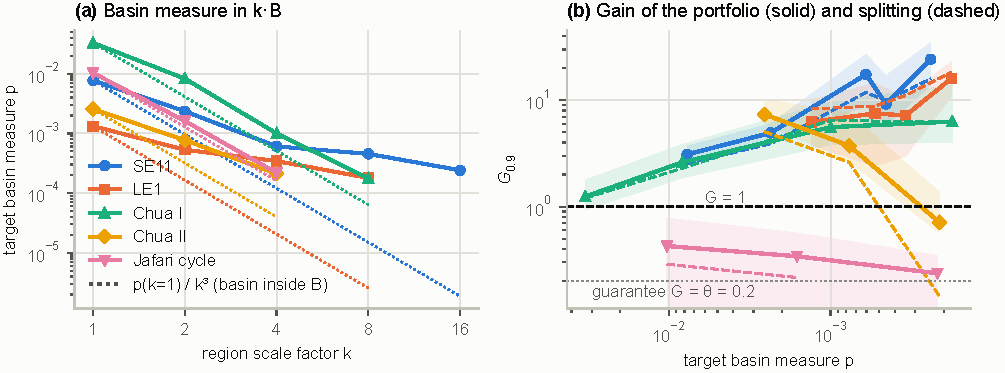
\includegraphics[width=\textwidth]{figures/fig27_enlarged_regions.pdf}
\caption{Real systems in enlarged regions $kB$. (a) Basin measure of the hidden target versus $k$; dotted lines: $p_{k=1}/k^3$, the measure if the basin lay inside $B$. (b) Gain of the portfolio (solid, with 95\% intervals) and of splitting (dashed) versus the basin measure, which decreases to the right. Dashed horizontal line: $G=1$; dotted: the guarantee $G=\theta=0.2$.}
\label{fig:enlarged}
\end{figure*}

\section{Discretization limit at very small \texorpdfstring{$p$}{p}}\label{app:smallp}

Figure~\ref{fig:smallp} shows the gain on D2 down to $p=10^{-7}$ and the diagnostic variants. Two alternative explanations of the breakdown below $p=10^{-5}$ were ruled out. Lowering the step floor of the splitting chains tenfold, or removing it, leaves every run unchanged: the floor is never reached. A second move that redraws a random subset of coordinates from the uniform distribution, akin to the componentwise Metropolis algorithm of the original subset simulation,\cite{AuBeck2001} helps only partly: at $p=10^{-6}$, splitting then succeeds in 50\% of runs and the portfolio in 68\%, but at $10^{-7}$ there is still no gain. The same move doubles the gain at $p=10^{-4}$ (53 for splitting and 35 for the portfolio); it is a natural extension of the method but is not used elsewhere in this paper. Reducing the integration step restores the order-of-growth gain, as stated in Sec.~\ref{sec:scaling_p}; these gains are counted in integrations, each of which is 4 or 16 times longer, so the gain in computing time is correspondingly smaller; the test demonstrates the mechanism, not a practical speedup. The level threshold also explains why one informative point is not enough: the level $\xi_l$ is the tenth largest value in the reference sample, and when fewer than ten points are informative, the threshold is $\xi_l=0$ (all escapes at the first step tie), the selection is empty, and the chains restart; the gain at $p=10^{-5}$ is carried by the runs whose reference sample contains several informative points. Figure~\ref{fig:scaln} shows the dependence on dimension at fixed $p=10^{-4}$.

\begin{figure}
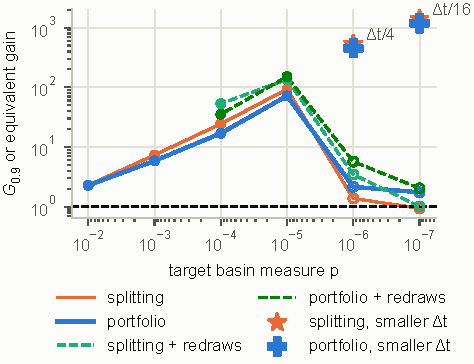
\includegraphics[width=\columnwidth]{figures/fig29_d2_small_p.pdf}
\caption{Family D2 ($n=6$): gain down to $p=10^{-7}$. Filled markers: $G_{0.9}$; open markers: equivalent gain $-\ln(1-f)/(pN_{\max})$ from the fraction $f$ of runs that found the target within the budget $N_{\max}$. Dashed lines: the variant with an additional move that redraws a random subset of coordinates (the variants with a lowered step floor coincide with the base curves and are not shown). Stars and crosses: splitting and the portfolio with the integration step reduced 4 times ($p=10^{-6}$) and 16 times ($p=10^{-7}$), with $N^0_{0.9}=\ln10/p$.}
\label{fig:smallp}
\end{figure}

\begin{figure}
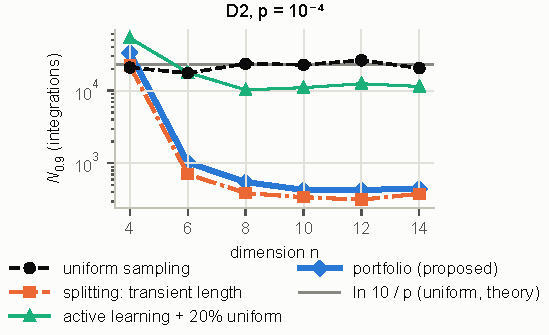
\includegraphics[width=\columnwidth]{figures/fig24_scaling_n.pdf}
\caption{Detection cost versus the phase-space dimension (family D2, $p=10^{-4}$, $R=100$). Dashed line: $\ln10/p$. At $n=4$, the reaction coordinate is uninformative because of the discretization limit; for $n\ge6$, the portfolio gain is 17--61 times.}
\label{fig:scaln}
\end{figure}

\section{Channel diagnostics}\label{app:diagnostics}

The prediction of the cost model was tested on a uniform sample of $2\times10^4$ points per system (Fig.~\ref{fig:signal}). Channel B works when nontarget points with long transients converge spatially to the target. For Chua~II, the median distance $d(q)$ decreases with the upper-set fraction $q$ as $0.43\to0.19\to0.12$; for LE1, as $0.53\to0.22\to0.13$; for SE11, as $0.47\to0.19\to0.15$; and for D2, as $0.74\to0.60\to0.53$ (at $q=0.2$, 0.04, and 0.008); the splitting gain here is 2.5--8.3 times. For the Jafari cycle ($0.99\to1.35$) and for D1 ($1.26\to1.38\to1.41$), $d(q)$ grows, and there is no gain. At the same time, in D1, the fraction of the target in the upper sets grows: the regions of long trajectories are scattered, and there is no path to the target through them. The AUC of the coordinate $\xi$ alone (0.88--0.97 for all systems except the Jafari cycle, 0.61) does not separate these cases, whereas $d(q)$ does. For the Huynh map, there is a gradient over only one decade ($d$ drops to 0.22 and grows again); at $p\approx0.009$, it barely pays back the initial sample and the levels.

\begin{figure}
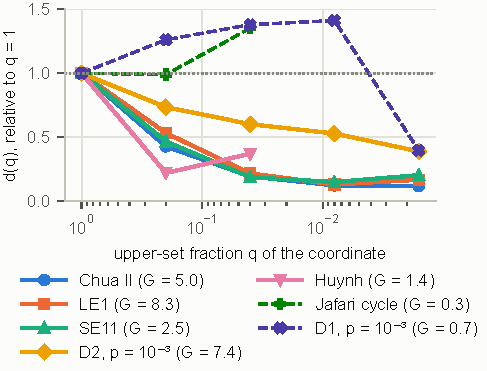
\includegraphics[width=\columnwidth]{figures/fig26_signal_curves.pdf}
\caption{Diagnostics of channel B from a uniform sample: the median distance from nontarget points of the upper set of the coordinate $\xi$ to the target (normalized to the value at $q=1$) versus the fraction $q$, which decreases to the right. A decreasing $d(q)$ (solid: Chua~II, LE1, SE11, D2) comes with a splitting gain (Tables~\ref{tab:gains} and \ref{tab:scaling}), and an increasing one (dashed: Jafari cycle, D1) with its absence.}
\label{fig:signal}
\end{figure}

\section{Implementation details of the two-stage configuration}\label{app:implementation}

The own computations of the arms (nearest-neighbor queries of the active-learning arm, the chains, and the matching) take 1--8\% of the wall time on the Chua systems with up to two copies, 28\% on three uncoupled copies of Chua~II, and 20--60\% on the cheap problems, where an integration costs microseconds. Brute-force neighbor search for $n\ge6$ reduces the queries by a factor of 1.6--2.6 relative to a tree ($G_T$ from 16 to 29 on three coupled copies of SE11). The cap on the training sample of the classifier (the last $2\times10^4$ evaluated points) removes the growth of the overhead in long runs: on three uncoupled copies of Chua~II, it lowers the overhead from 51\% to 28\% and, by training the classifier on recent points only, also lowers the median cost from $1.4\times10^5$ to $8.6\times10^4$ integrations and raises the number of runs that succeed within $4\times10^5$ integrations from 8 to 9 of 10. A wider batch, with two or four times more chains and boundary points to occupy more cores, does not pay: the number of evaluations grows by a factor of 1.5--3, whereas the time per evaluation decreases by about 10\% only. The gains in time of Table~\ref{tab:cost} were measured with four threads per process and those of Table~\ref{tab:time} on one thread; with the batch of 500 evaluations used here, the portfolio parallelizes better than uniform sampling (its time to detection falls 4.0-fold from one to four threads on the coupled Chua circuits, against 1.6-fold for the cost per uniform evaluation), so the four-thread gains are larger, and the one-thread values are the conservative ones.
